\subsubsection{Cenário com Vento em X (WindX)}

Neste cenário, o objetivo é analisar o comportamento do quadricóptero sob a influência de uma rajada de vento na direção \(X\). Essa análise permite observar como o sistema de controle lida com perturbações externas no eixo \(X\), tanto em termos de estabilidade quanto de capacidade de retornar à posição desejada.

\begin{figure}[H]
    \centering
    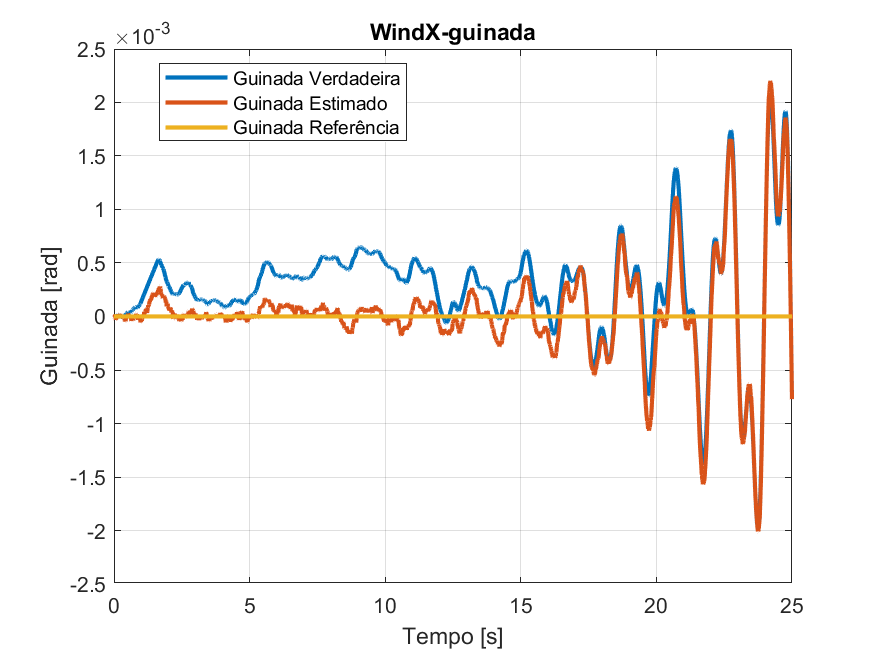
\includegraphics[width=1\textwidth]{WindX-guinada.png}
    \caption{Comportamento da Guinada sob Vento em X}
    \label{fig:WindX-guinada}
\end{figure}

A Figura \ref{fig:WindX-guinada} mostra a resposta da guinada do quadricóptero ao vento em \(X\). Observa-se que o ângulo de guinada real (\textbf{Guinada Verdadeira}) apresenta variações significativas, enquanto a guinada estimada se mantém próxima da referência, indicando uma tentativa de manter a orientação desejada. Esse comportamento sugere que o sistema de controle tenta corrigir as perturbações, mas enfrenta dificuldades em eliminar completamente os efeitos do vento.

\begin{figure}[H]
    \centering
    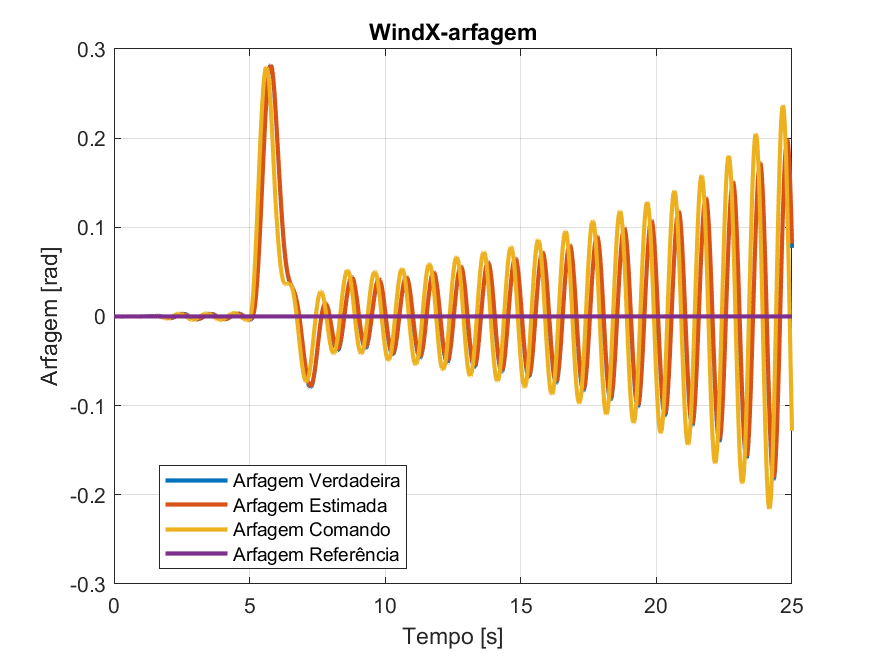
\includegraphics[width=1\textwidth]{WindX-arfagem.png}
    \caption{Comportamento da Arfagem sob Vento em X}
    \label{fig:WindX-arfagem}
\end{figure}

Na Figura \ref{fig:WindX-arfagem}, observa-se o ângulo de arfagem. As oscilações crescentes na arfagem verdadeira sugerem uma resposta oscilatória e instável do sistema ao longo do tempo, enquanto a arfagem estimada acompanha esse comportamento, mas não consegue eliminá-lo totalmente. Esse fenômeno indica que o controlador de arfagem é impactado significativamente pelo vento, possivelmente necessitando de ajustes nos ganhos para melhorar o amortecimento.

\begin{figure}[H]
    \centering
    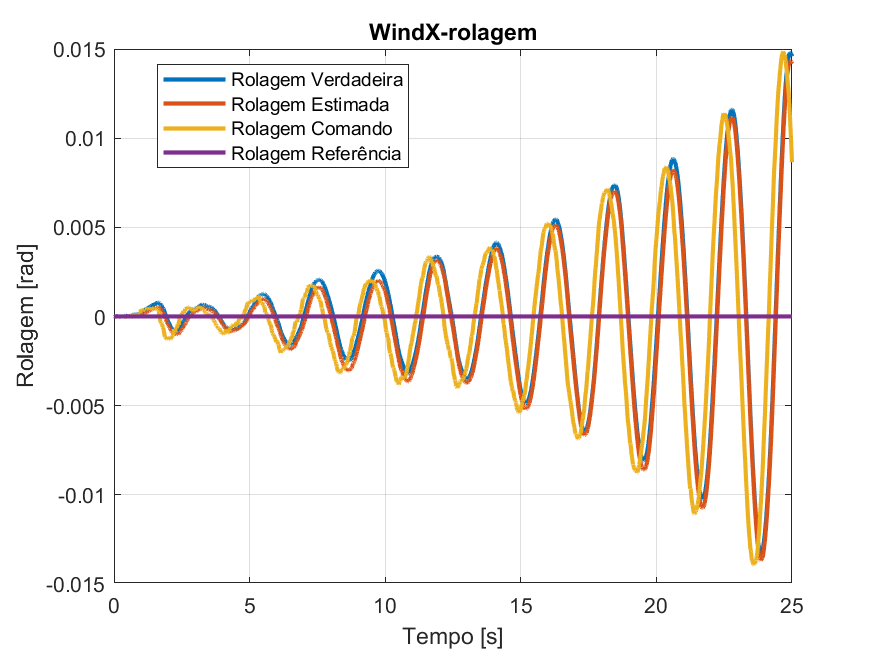
\includegraphics[width=1\textwidth]{WindX-rolagem.png}
    \caption{Comportamento da Rolagem sob Vento em X}
    \label{fig:WindX-rolagem}
\end{figure}

A Figura \ref{fig:WindX-rolagem} exibe a rolagem. A resposta segue um padrão oscilatório semelhante ao observado na arfagem, com oscilações que aumentam progressivamente ao longo do tempo. Esse comportamento indica que a rolagem também é sensível às perturbações, e o sistema de controle apresenta dificuldades em amortecer essas oscilações.

\begin{figure}[H]
    \centering
    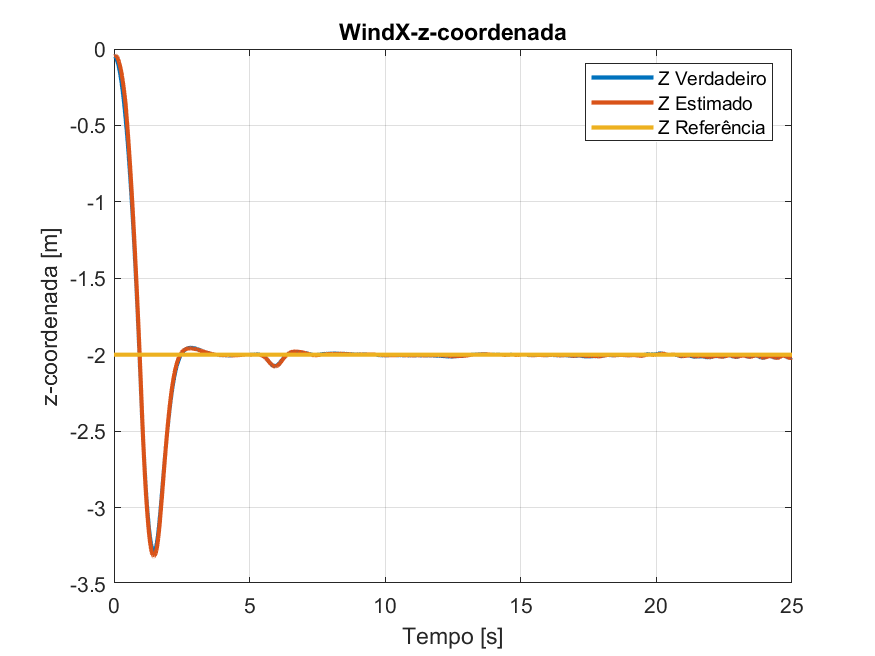
\includegraphics[width=1\textwidth]{WindX-z-coordenada.png}
    \caption{Comportamento da Coordenada Z sob Vento em X}
    \label{fig:WindX-z-coordenada}
\end{figure}

Na Figura \ref{fig:WindX-z-coordenada}, observa-se a resposta em \(Z\). A coordenada \(Z\) verdadeira e estimada se mantêm relativamente estáveis após um leve overshoot inicial, sugerindo que o controle de altitude não é diretamente afetado pela rajada de vento em \(X\).

\begin{figure}[H]
    \centering
    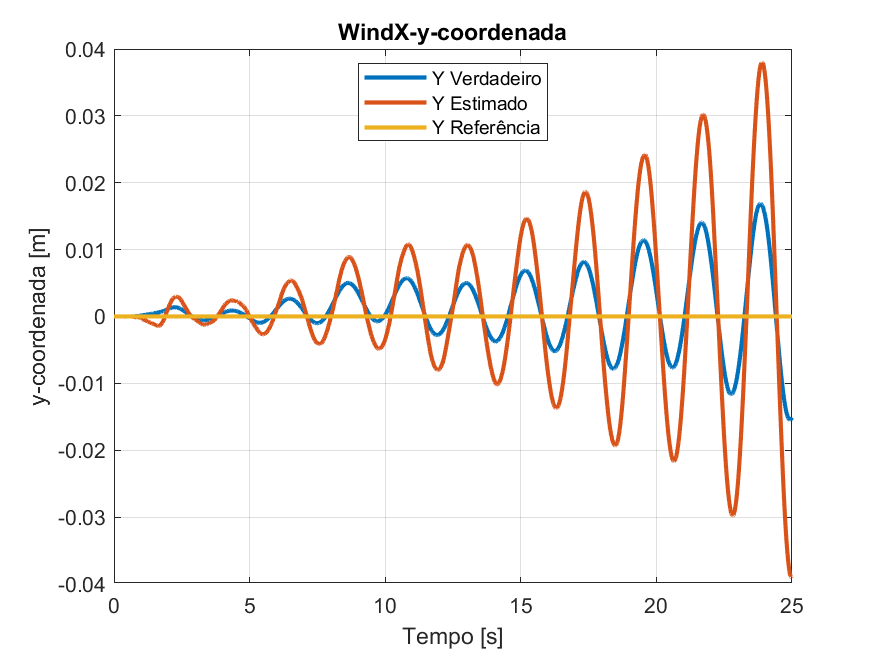
\includegraphics[width=0.45\textwidth]{WindX-y-coordenada.png}
    \hfill
    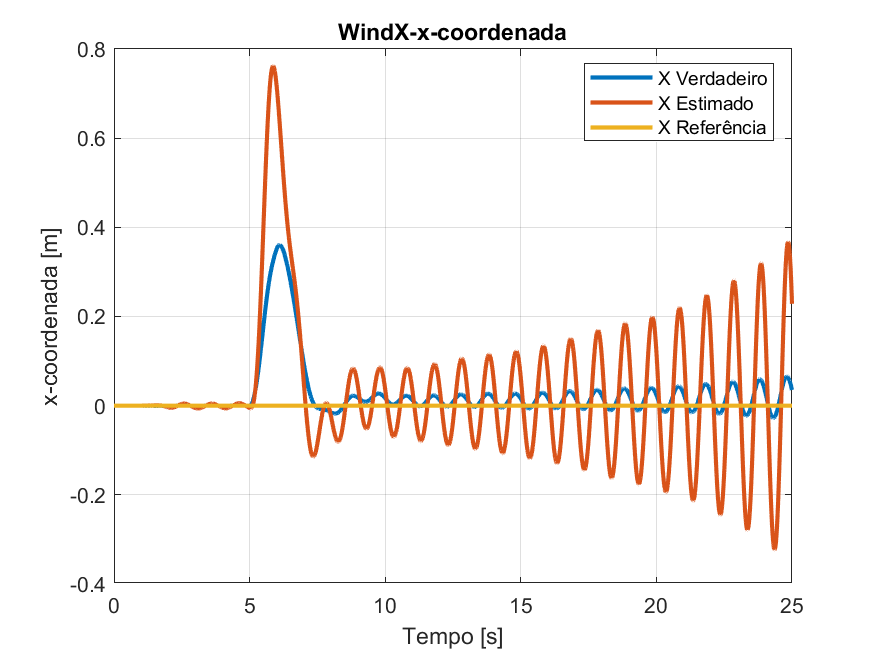
\includegraphics[width=0.45\textwidth]{WindX-x-coordenada.png}
    \caption{Comportamento das Coordenadas X e Y sob Vento em X}
    \label{fig:WindX-x-y-coordenada}
\end{figure}

As Figuras \ref{fig:WindX-x-y-coordenada} mostram as respostas em \(X\) e \(Y\). Em \(X\), o sistema apresenta uma resposta oscilatória crescente, indicando uma instabilidade em resposta ao vento. Em \(Y\), as oscilações são também visíveis, o que indica que a rajada de vento em \(X\) provoca um acoplamento indesejado nos eixos laterais, afetando a estabilidade geral do quadricóptero.

%\subsubsection*{Conclusão}

%A análise do cenário com vento em \(X\) evidencia que o sistema de controle do quadricóptero possui limitações ao lidar com perturbações externas. As respostas oscilatórias e instáveis nas coordenadas \(X\), \(Y\), e nos ângulos de arfagem e rolagem sugerem que ajustes no controlador são necessários, especialmente para melhorar o amortecimento e a resistência a perturbações. Uma recomendação seria aumentar o ganho derivativo (\(K_d\)) para tentar reduzir as oscilações e obter uma resposta mais estável.


%---------------------------------------------------------------------
% INDICE REMISSIVO
%---------------------------------------------------------------------
\phantompart
\printindex
%---------------------------------------------------------------------
